%!TEX root = ../../../main.tex

\subsection{Experimental results on MICAGes dataset}

    \paragraph{1) Cross-view validation:} It can be seen in Table.\ref{tab:mica_cross} that pc-MvDA outperforms in almost every cases. With the first protocol, the norm accuracy of pc-MvDA of 74.52\% surpasses that of MvDA-vc (72.12\%) by 2.4\% and that of MvDA (64.94\%) by a large margin of 9.58\%. Especially in case of C3D features, the proposed algorithm achieved 90.2\% recognition rate whereas MvDA returns only 67.13\%.

    \begin{table}[htbp]
    \centering
    \caption{Cross-view recognition comparison on MICAGes dataset.}
    \resizebox{0.8\textwidth}{!}{
    \begin{tabular}{|c|c|c|c|c|c|c|}
        \hline
        \multirow{2}{*}{Deep features}          & \multicolumn{3}{c|}{Protocol 1}          & \multicolumn{3}{c|}{Protocol 2}            \\ \cline{2-7} 
                                                & MvDA  & MvDA-vc        & pc-MvDA         & MvDA  & MvDA-vc        & pc-MvDA           \\ \hline
        \multicolumn{1}{|c|}{C3D}               & 67.13 & 85.98          & \textbf{90.20}  & 93.74 & 99.80          & \textbf{100}      \\ \hline
        \multicolumn{1}{|c|}{ResNet-50 3D}      & 94.91 & 95.25          & \textbf{95.62}  & 97.43 & \textbf{99.97} & 99.79             \\ \hline
        \multicolumn{1}{|c|}{ResNet-50 RNN}     & 58.01 & 61.64          & \textbf{64.13}  & 100   & 100            & 100               \\ \hline
        \multicolumn{1}{|c|}{ResNet-50 TA}      & 53.58 & \textbf{59.55} & 58.62           & 96.70 & 99.48          & \textbf{99.83}    \\ \hline
        \multicolumn{1}{|c|}{ResNet-50 AP}      & 51.07 & 58.19          & \textbf{64.04}  & 99.73 & \textbf{99.99} & 99.89             \\ \hline
    \end{tabular}}
    \label{tab:mica_cross}
    \end{table}

    %Table.\ref{tab:cross_feature_mica} compares all types of deep features regarding accuracy of the proposed algorithm. 
    The top ranking of features applies identically and radically proves the superiority of 3D convolution based clip-level feature extraction in video recognition: ResNet-50 3D at 95.62\% and C3D at 90.2\%. The rest are ResNet-50 RNN (64.13\%), ResNet-50 AP (64.04\%) and ResNet-50 TA (58.62\%). For the second protocol, MvDA-vc (99.85\%) and pc-MvDA (99.9\%) are nearly even in performance while MvDA achieved 97.52\%.

    \begin{table}[htbp]
    \centering
    \caption{Cross-view recognition results of different features on MICAGes dataset with pc-MvDA method. The result in the bracket are accuracies of using features C3D, ResNet-50 3D, ResNet-50 RNN, ResNet-50 TA, RestNet-50 AP respectively. Each row corresponds to training view (from view K1 to view K5). Each column corresponds to testing view (from view K1 to view K5).}
    \resizebox{\textwidth}{!}{\begin{tabular}{|c|c|c|c|c|c|}
        \hline
        \backslashbox{Training}{Testing} & K1 & K2 & K3 & K4 & K5 \\ \hline
        K1 & N/A & \begin{tabular}{@{}c@{}} (92.9, \textbf{95.5}, 69.4, \\ 63.9, 65.1) \end{tabular} & \begin{tabular}{@{}c@{}} (93.7, \textbf{98.0}, 79.1, \\ 75.8, 74.7) \end{tabular} & \begin{tabular}{@{}c@{}} (90.5, \textbf{97.6}, 64.5, \\ 68.8, 70.8) \end{tabular} & \begin{tabular}{@{}c@{}} (89.2, \textbf{92.6}, 56.0, \\ 43.7, 58.2) \end{tabular} \\ \hline       
        K2 & \begin{tabular}{@{}c@{}} (84.7, \textbf{94.6}, 51.3, \\ 41.4, 53.7) \end{tabular} & N/A & \begin{tabular}{@{}c@{}} (94.6, \textbf{97.6}, 78.9, \\ 75.4, 77.5) \end{tabular} & \begin{tabular}{@{}c@{}} (91.3, \textbf{97.6}, 64.4, \\ 68.5, 68.0) \end{tabular} & \begin{tabular}{@{}c@{}} (87.4, \textbf{92.7}, 56.1, \\ 42.0, 55.6) \end{tabular} \\ \hline       
        K3 & \begin{tabular}{@{}c@{}} (87.5, \textbf{94.9}, 51.9, \\ 43.6, 52.7) \end{tabular} & \begin{tabular}{@{}c@{}} (93.0, \textbf{95.5}, 70.1, \\ 64.7, 63.4) \end{tabular} & N/A & \begin{tabular}{@{}c@{}} (90.0, \textbf{97.6}, 63.2, \\ 62.6, 67.5) \end{tabular} & \begin{tabular}{@{}c@{}} (88.9, \textbf{92.2}, 57.2, \\ 41.8, 56.6) \end{tabular} \\ \hline       
        K4 & \begin{tabular}{@{}c@{}} (86.7, \textbf{94.7}, 50.8, \\ 48.9, 54.9) \end{tabular} & \begin{tabular}{@{}c@{}} (90.2, \textbf{95.5}, 71.5, \\ 68.2, 61.8) \end{tabular} & \begin{tabular}{@{}c@{}} (92.5, \textbf{98.0}, 81.0, \\ 76.0, 74.4) \end{tabular} & N/A & \begin{tabular}{@{}c@{}} (89.7, \textbf{92.3}, 54.3, \\ 44.9, 56.6) \end{tabular} \\ \hline       
        K5 & \begin{tabular}{@{}c@{}} (84.9, \textbf{94.9}, 48.4, \\ 41.5, 57.9) \end{tabular} & \begin{tabular}{@{}c@{}} (90.4, \textbf{95.5}, 72.6, \\ 64.1, 65.7) \end{tabular} & \begin{tabular}{@{}c@{}} (94.0, \textbf{97.8}, 79.1, \\ 72.5, 76.3) \end{tabular} & \begin{tabular}{@{}c@{}} (91.9, \textbf{97.3}, 62.7, \\ 64.1, 69.0) \end{tabular} & N/A \\ \hline
    \end{tabular}}
    \label{tab:cross_feature_mica}
    \end{table}

    \paragraph{2) Multi-view validation}: The multi-view recognition results in Table.\ref{tab:mica_multi} shows an almost alike trend for both protocols. In general, pc-MvDA is 8.95\% and 0.72\% higher in accuracy for protocol 1, and 2.75\% and 0.04\% for protocol 2, in comparison with MvDA and MvDA-pc respectively.

    % TODO
    In virtually every experiments of MICAGes and two earlier benchmark datasets, the proposed extension is superior. The average accuracies of pc-MvDA is, in comparison on protocol 1 (and protocol 2 resp.), 5.29\% (1.21\% resp.) higher than MvDA, 1.21\% (0.62\% resp.) better than MvDA-vc. Despite not being as intuitive and straightly intelligible as pairwise-covariance, the multi-view resemblance added in MvDA-vc achieved nearly the performance of pc-MvDA. However, this view-consistency can be easily splitted into pairwise terms and intergrated into the objective of pc-MvDA in future works for further analysis.

    \begin{table}[htbp]
    \centering
    \caption{Multi-view recognition comparison on MICAGes dataset.}
    \resizebox{0.8\textwidth}{!}{
    \begin{tabular}{|c|c|c|c|c|c|c|}
        \hline
        \multirow{2}{*}{Deep features}          & \multicolumn{3}{c|}{Protocol 1}          & \multicolumn{3}{c|}{Protocol2}                     \\ \cline{2-7} 
                                                & MvDA  & MvDA-vc        & pc-MvDA         & MvDA           & MvDA-vc       & pc-MvDA           \\ \hline
        \multicolumn{1}{|c|}{C3D}               & 68.31 & 87.70          & \textbf{89.99}  & 88.79          & 99.54         & \textbf{100}      \\ \hline
        \multicolumn{1}{|c|}{ResNet-50 3D}      & 95.32 & 95.26          & \textbf{95.54}  & \textbf{100}   & 99.96         & 99.80             \\ \hline
        \multicolumn{1}{|c|}{ResNet-50 RNN}     & 57.50 & 63.05          & \textbf{63.83}  & 99.90          & \textbf{100}  & 99.97             \\ \hline
        \multicolumn{1}{|c|}{ResNet-50 TA}      & 54.43 & \textbf{61.46} & 58.25           & 96.72          & 99.49         & \textbf{99.69}    \\ \hline
        \multicolumn{1}{|c|}{ResNet-50 AP}      & 50.93 & 60.20          & \textbf{63.66}  & \textbf{99.99} & 99.93         & 99.67             \\ \hline
    \end{tabular}}
    \label{tab:mica_multi}
    \end{table}

    In addition to the same propensity shown, MICAGes also reveals the robustness of 3D convolution to generate fine clustered private feature space because this dataset contains exclusively hand gestures, which take part in a relatively small region of the captured videos. ResNet-50 3D and C3D are predominant for discriminant common space construction and classification and distances other features (Figure \ref{fig:pc-MvDA_confusion_mica}).

    \begin{figure}[htbp]
        \centering
        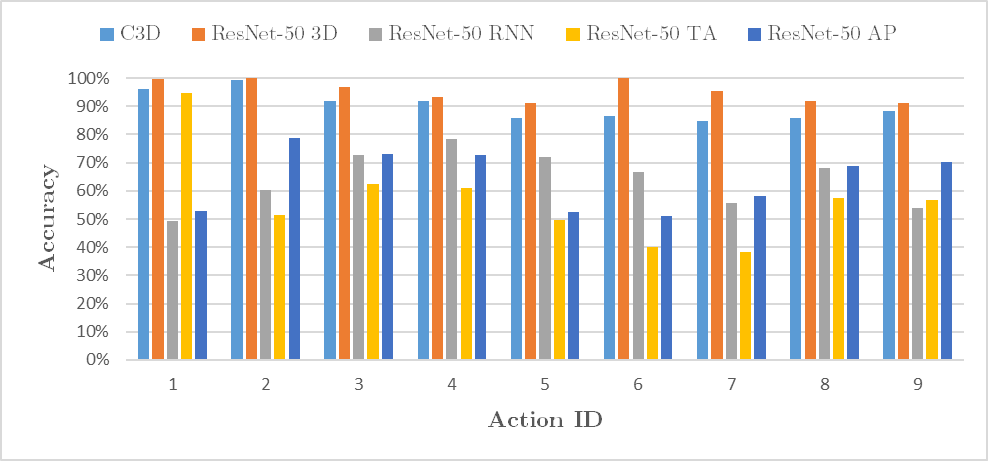
\includegraphics[width=0.8\linewidth]{figs/pc-MvDA_confusion_mica.png}
        \caption{Comparison of accuracy on each action class using different deep features combined with pc-MvDA on MICAGes dataset.}
        %\vspace{-0.3cm}
        \label{fig:pc-MvDA_confusion_mica}
    \end{figure}

    To better study the behavior of investigated multi-view analysis algorithms, t-SNE embedding of original private spaces, MvDA and pc-MvDA common space generated by protocol 1 are plotted in Figure \ref{fig:mica-tsne}. In these scatter plots, colors denote action classes, shapes as different views and train/test data are distinguished by border type. They explicitly denotes the surpassing capability of the proposed algorithm in finding a common space with prominent extra-class discrepancy. The data samples involved in training process are generally clustered in compact and separated blobs while testing data samples dissolve nearby. The better convergence of pc-MvDA compared to the baseline is usually only visible for harder features, whereas with the inputs of ResNet-50 3D features, which are already highly discriminated in private spaces, the improvement of pc-MvDA is negligible. Note that these illustrations of t-SNE embedding do not strictly depict an identical distribution of data.

    \begin{figure}[htbp]
        \centering
        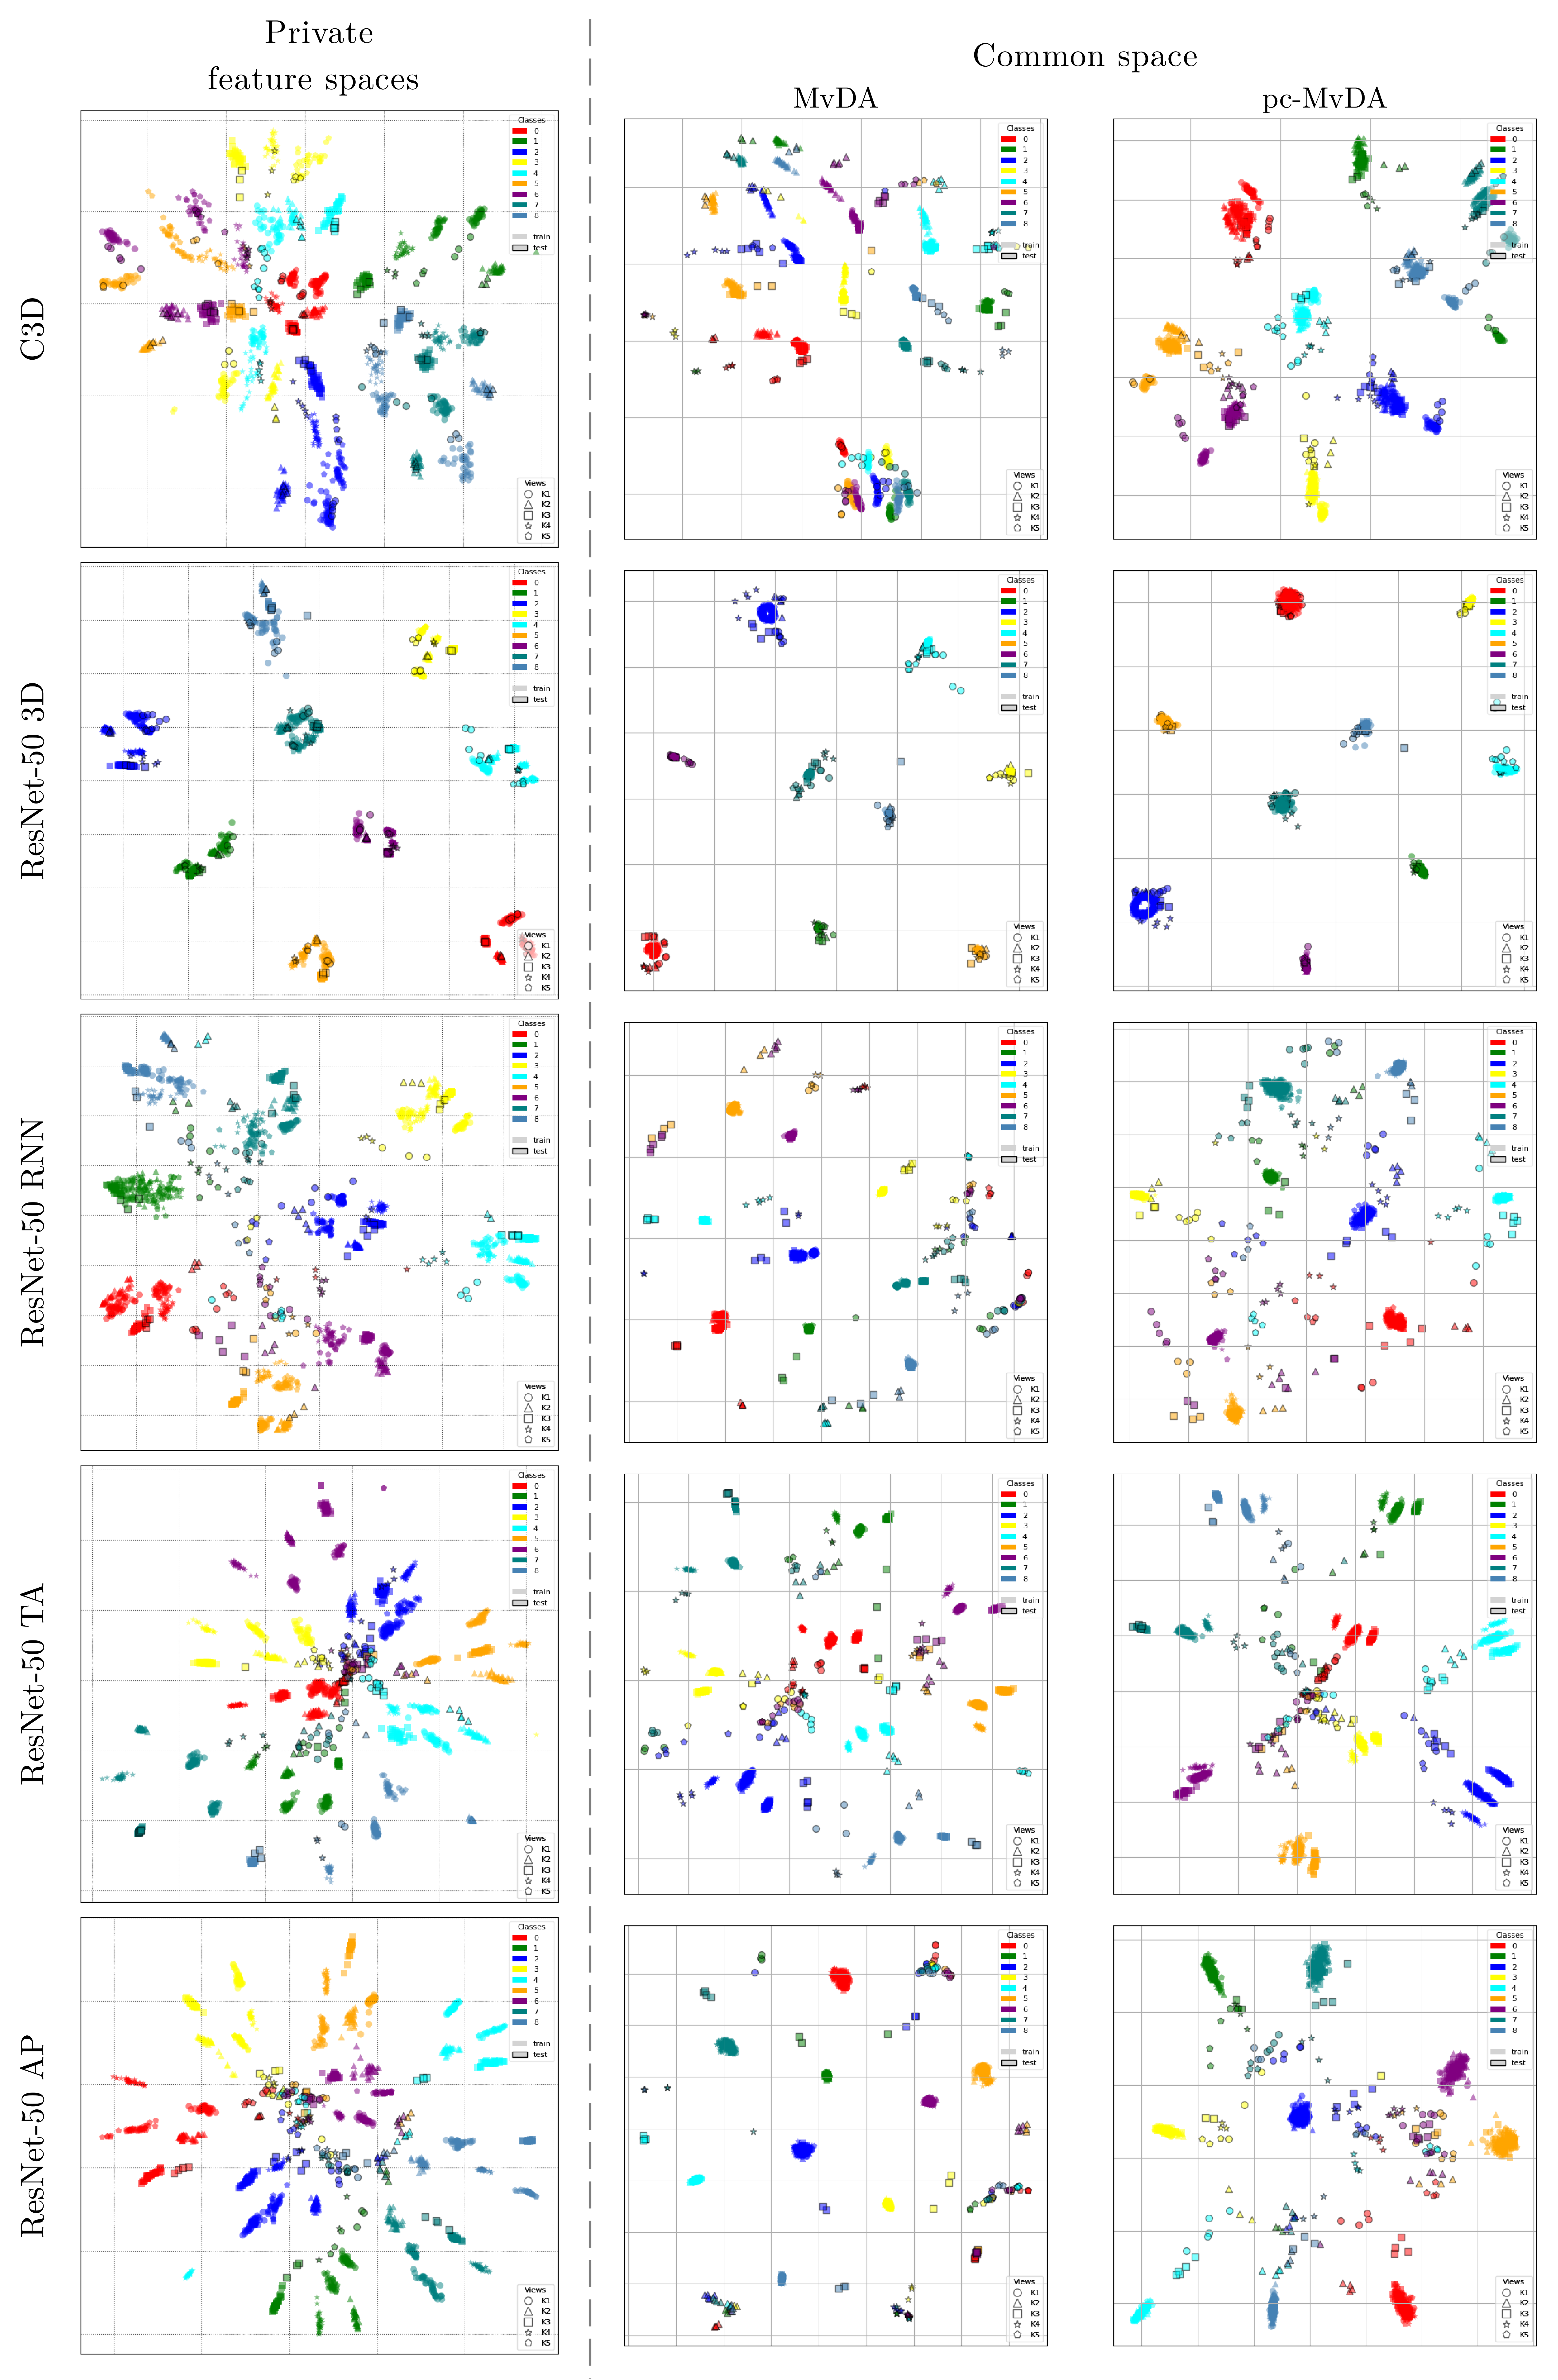
\includegraphics[width=1\linewidth, height=0.6\pdfpageheight, keepaspectratio=false]{figs/mica-tsne.png}
        \caption{First column: private feature spaces stacked and embedded together in a same coordinate system; Second column: MvDA common space; Third column: pc-MvDA common space.}
        %\vspace{-0.3cm}
        \label{fig:mica-tsne}
    \end{figure}
